\chapter{Конструкторский раздел}

В данном разделе формализована структура разработанного метода,
описана алгоритмическая основа функциональных блоков и их взаимодействия в рамках единой системы.

Структура решения представлена в виде IDEF0--диаграммы и подробных схем для каждого этапа обработки:
предварительной подготовки изображений, сегментации, оценки освещения, разделения альбедо и затенения,
расчета нормалей к поверхности и итогового восстановления трехмерной информации.

\section{IDEF-0 диаграммы}

На рисунке~\ref{idef0-a0} представлена диаграмма IDEF0 уровня A0 разработанного метода.

% TODO убрать из А0 управление метрики качества + добавить параметры алгоритмов к управлению на А1

\begin{figure}[H]
    \centering
    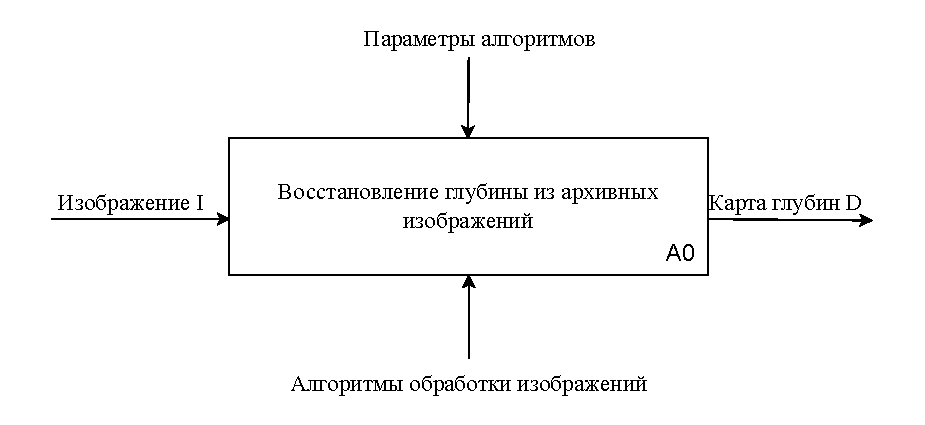
\includegraphics[scale=0.8]{img/IDEFA0}
    \caption{IDEF0-диаграмма уровня A0}
    \label{idef0-a0}
\end{figure}

Диаграмма нулевого уровня представляет всю систему как единый блок с указанием входов, выходов, управления и механизмов.
Входными данными системы являются архивные фотографии, выходными --- восстановленная карта глубин.

На рисунке~\ref{idef0-a1} показана декомпозиция функционального блока A0, детализирующая основные процессы обработки изображений.

\begin{figure}[H]
    \centering
    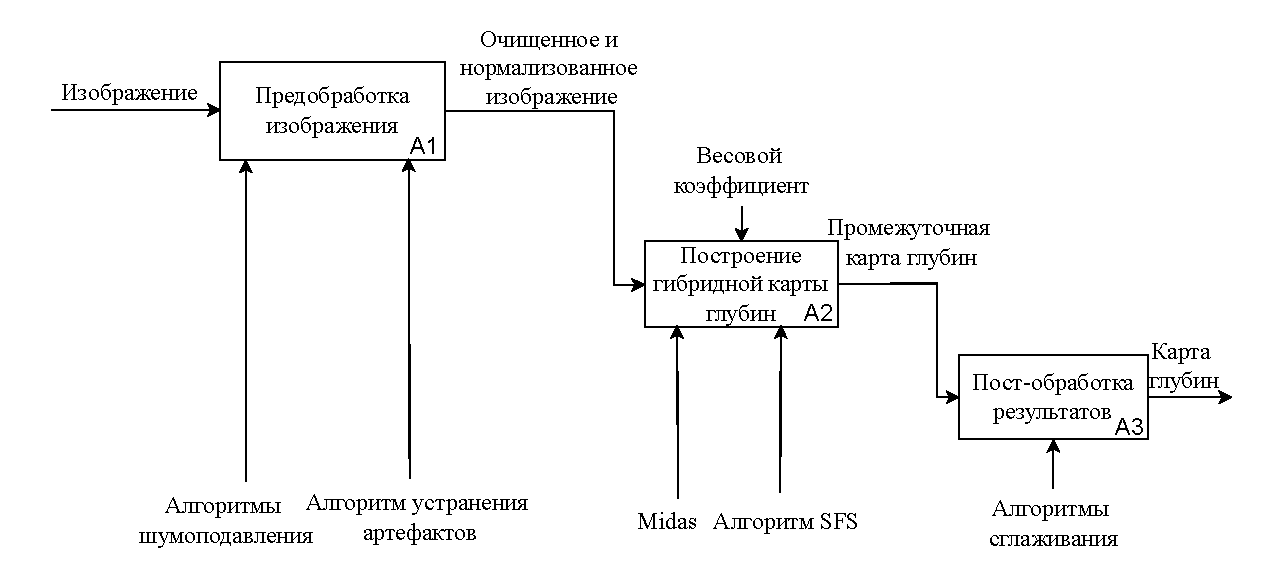
\includegraphics[scale=0.8]{img/IDEFA1}
    \caption{IDEF0-диаграмма уровня A1}
    \label{idef0-a1}
\end{figure}

Диаграмма уровня A1 визуализирует три основных функциональных блока системы: предобработка, гибридное восстановление и постобработка.
Отражены их взаимосвязи, потоки данных между блоками, управляющие воздействия и используемые механизмы.

%Рисунок~\ref{idef0-a2} демонстрирует декомпозицию второго блока диаграммы A1 --- процесса гибридного восстановления.
%
%\begin{figure}[H]
%    \centering
%    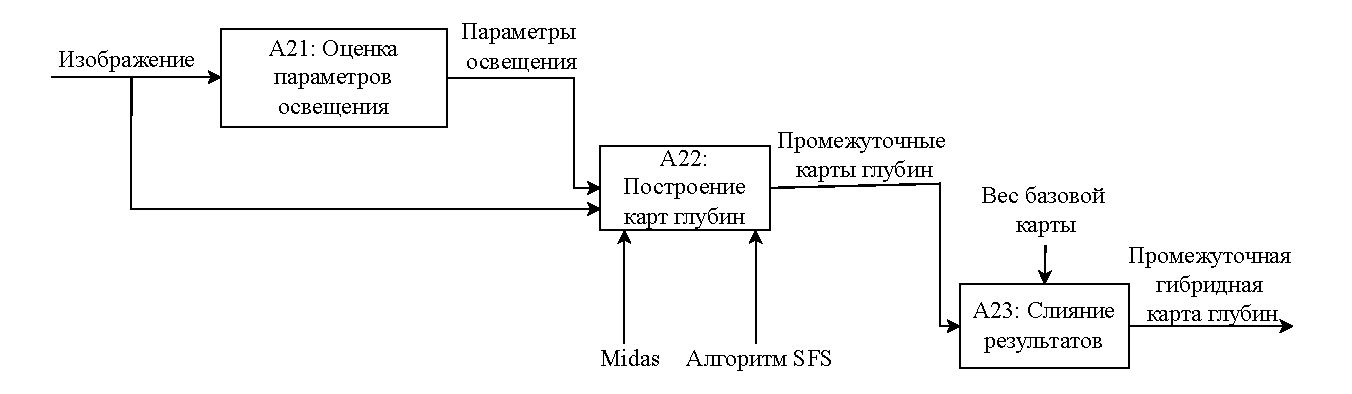
\includegraphics[scale=0.8]{img/IDEFA2}
%    \caption{IDEF0-диаграмма уровня A2}
%    \label{idef0-a2}
%\end{figure}
%
%На диаграмме уровня A2 детализирован процесс гибридного восстановления, включающий сегментацию изображения,
%оценку освещения, применение нейросетевого метода и метода Shape from Shading, а также интеграцию результатов.
%На этом этапе формируются ключевые промежуточные представления для каждого из используемых методов.

\section{Схемы алгоритмов}

На рисунке~\ref{preobr} представлена схема предварительной обработки входного изображения, включающая методы шумоподавления, нормализации освещения и коррекции артефактов, характерных для архивных фотографий.

\begin{figure}[H]
    \centering
    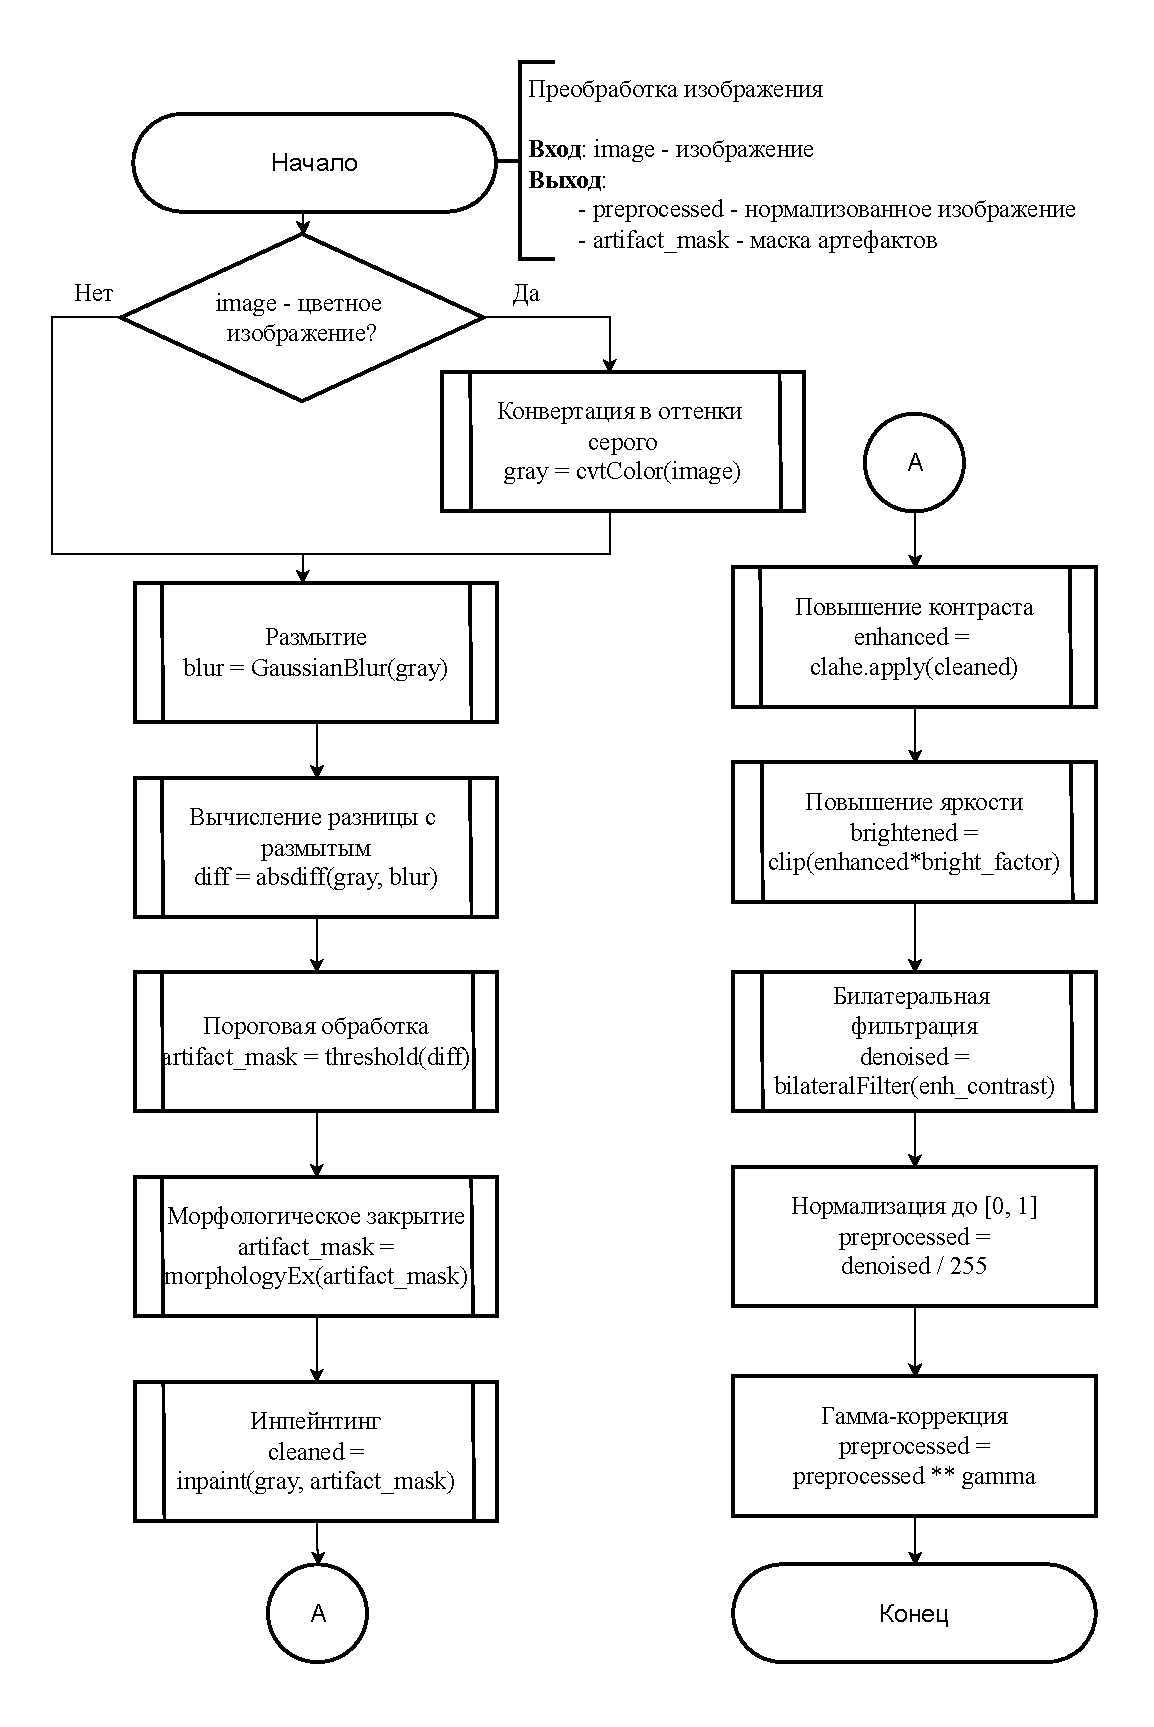
\includegraphics[scale=0.7]{img/preobr}
    \caption{Преобработка изображения}
    \label{preobr}
\end{figure}


Рисунок~\ref{reconstr} иллюстрирует основной алгоритм извлечения глубины, который объединяет нейросетевой метод для первичной оценки глубины с последующим уточнением деталей.

\begin{figure}[H]
    \centering
    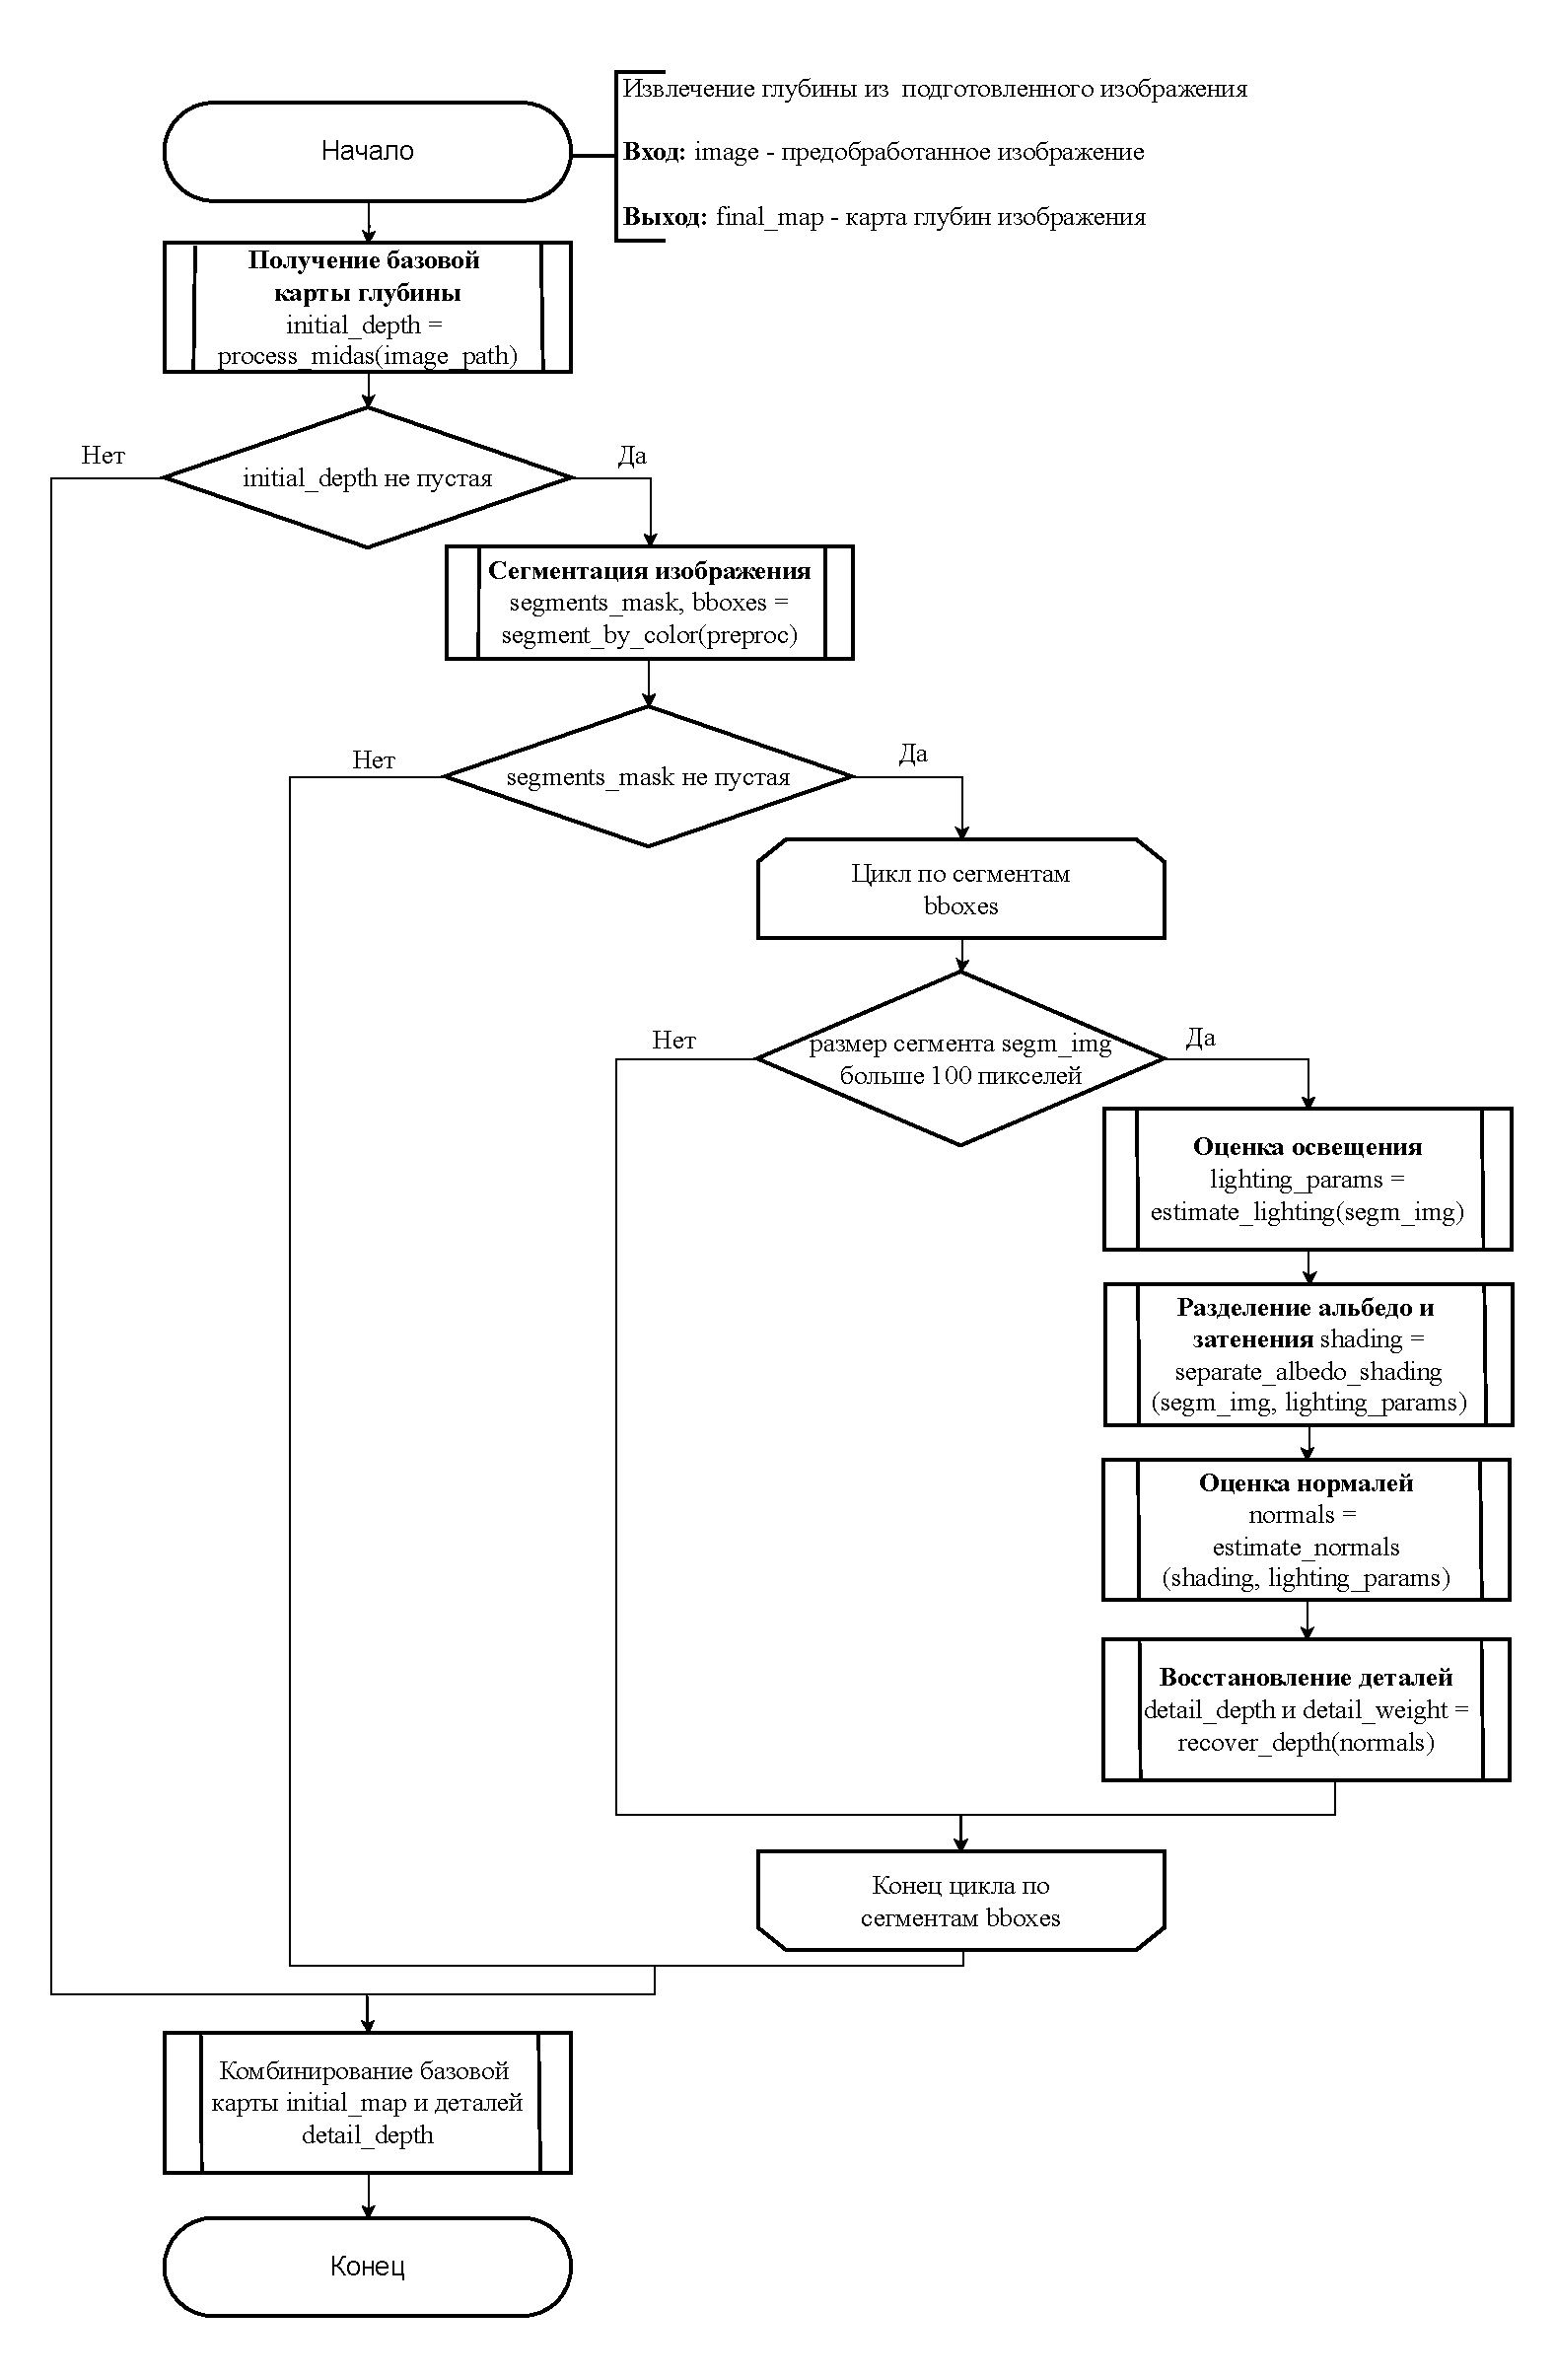
\includegraphics[scale=0.6]{img/reconstr}
    \caption{Извлечение глубины из подготовленного изображения}
    \label{reconstr}
\end{figure}

Схема на рисунке~\ref{segmentation} отражает процесс сегментации изображения, позволяющий выделить различные объекты сцены для их дальнейшей раздельной обработки методом Shape From Shading.

\begin{figure}[H]
    \centering
    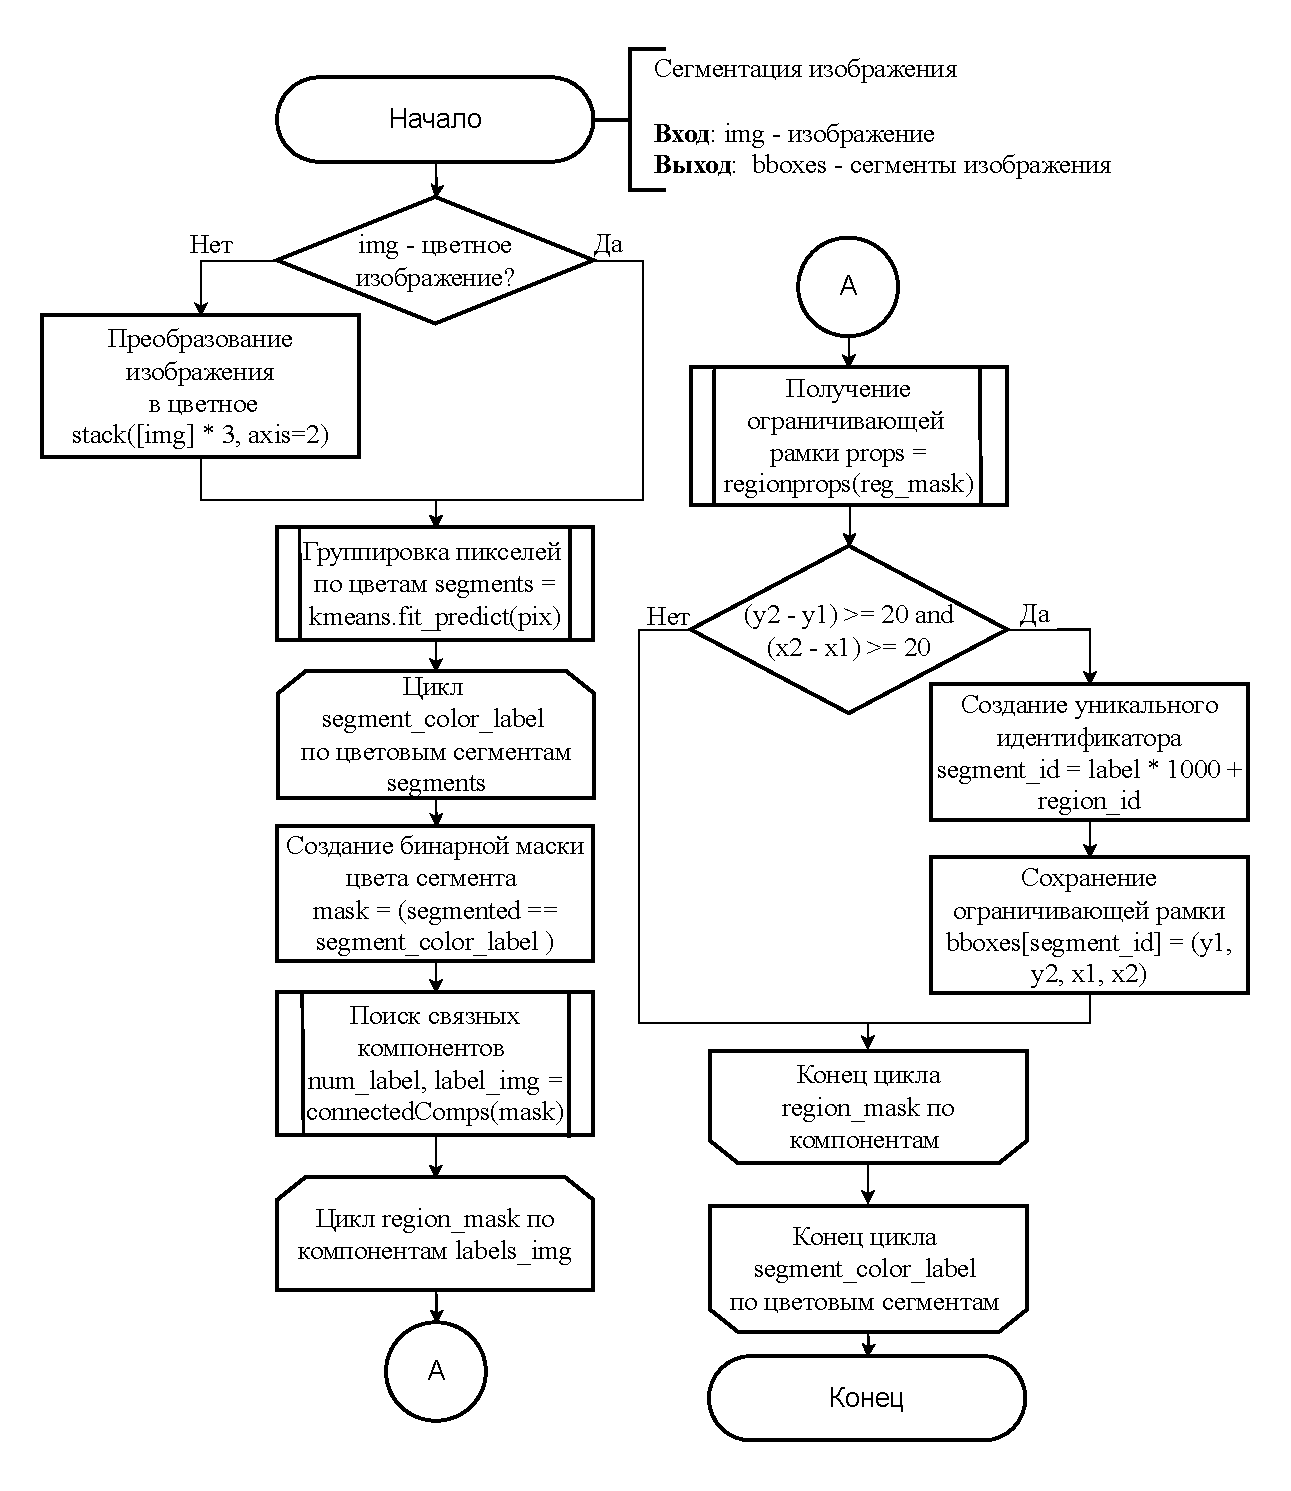
\includegraphics[scale=0.7]{img/segmentation}
    \caption{Сегментация изображения}
    \label{segmentation}
\end{figure}

На рисунке~\ref{light} представлен алгоритм оценки параметров освещения сцены, необходимых для корректного применения метода Shape from Shading.

\begin{figure}[H]
    \centering
    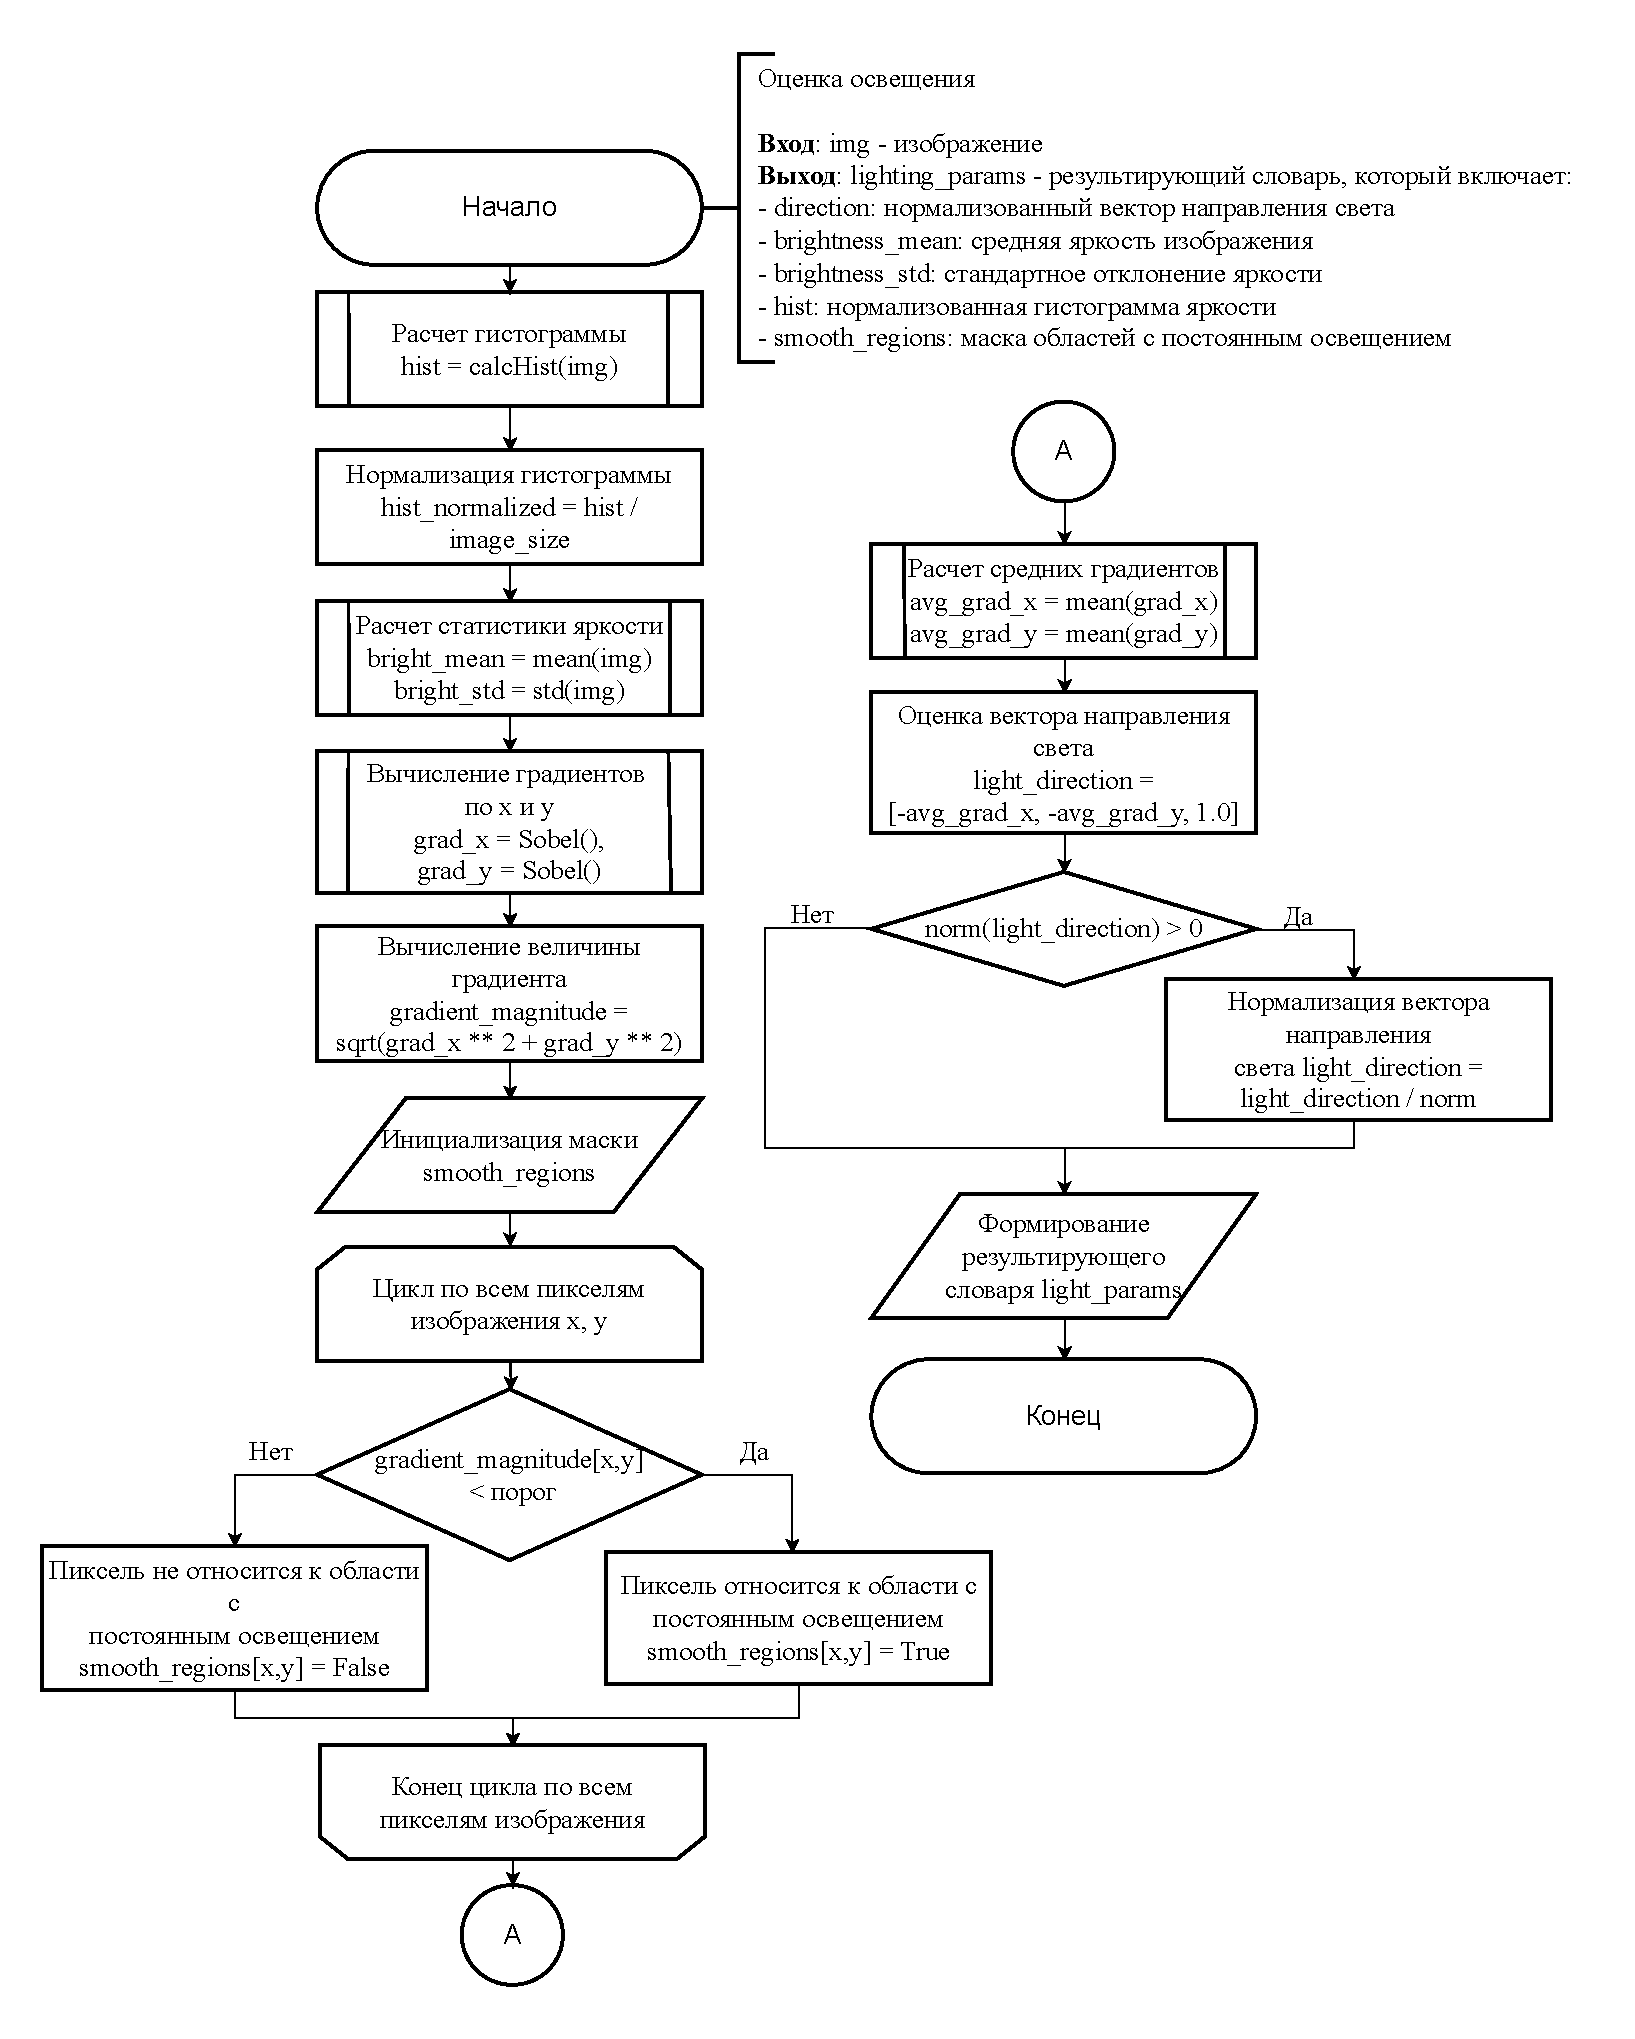
\includegraphics[scale=0.6]{img/light}
    \caption{Оценка освещения}
    \label{light}
\end{figure}

Рисунок~\ref{albedo} демонстрирует процесс разделения альбедо и затенения метода Shape from Shading, позволяющий отделить собственные цвета поверхностей от эффектов освещения.

\begin{figure}[H]
    \centering
    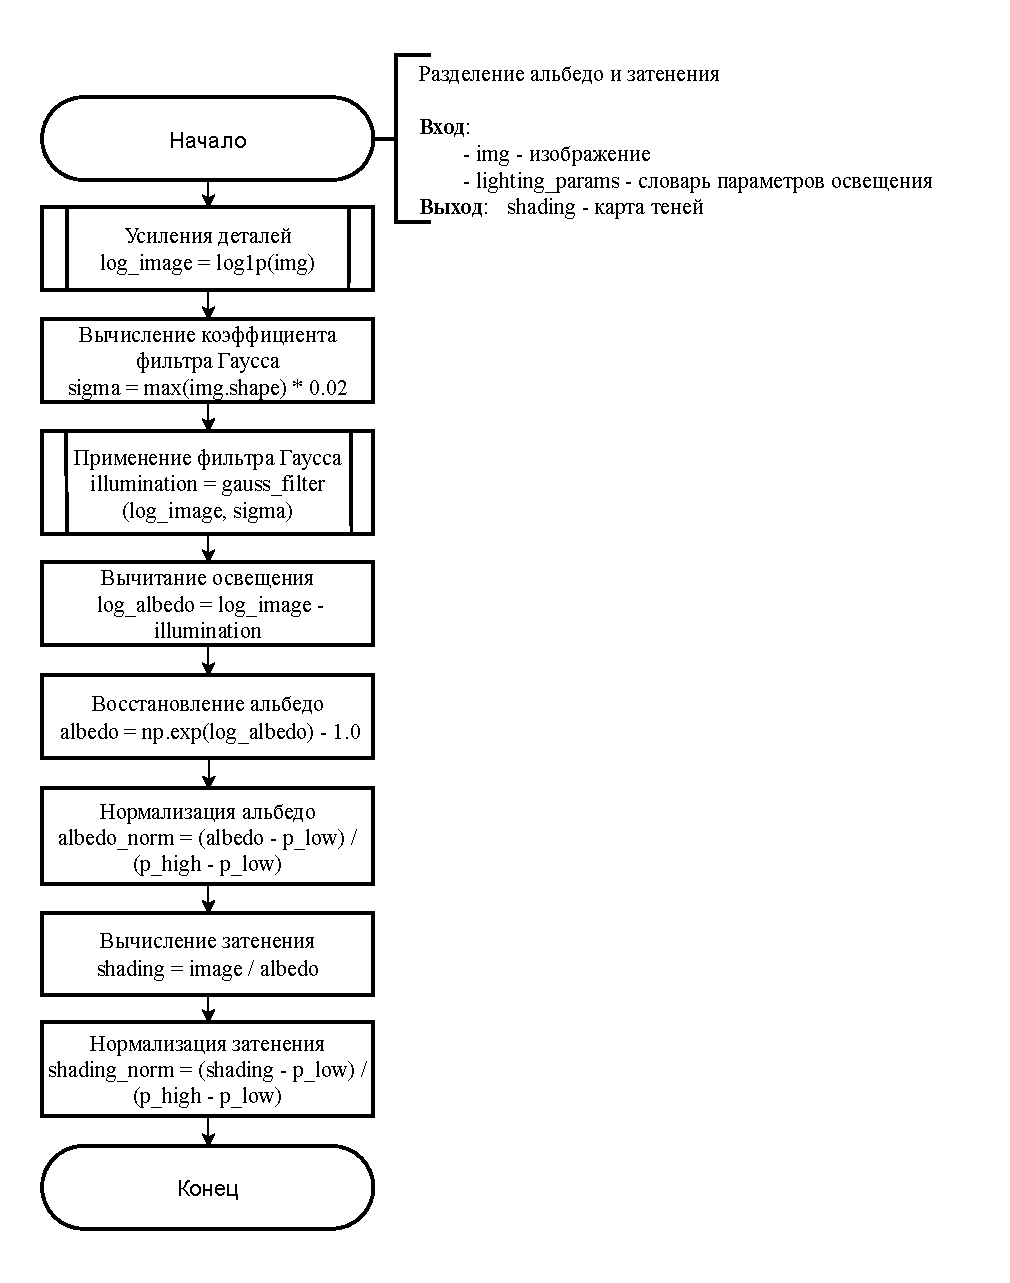
\includegraphics[scale=0.9]{img/albedo}
    \caption{Разделение альбедо и затенения}
    \label{albedo}
\end{figure}

Схема на рисунке~\ref{normals} описывает алгоритм вычисления нормалей к поверхности на основе полученного разделения альбедо и затенения.

\begin{figure}[H]
    \centering
    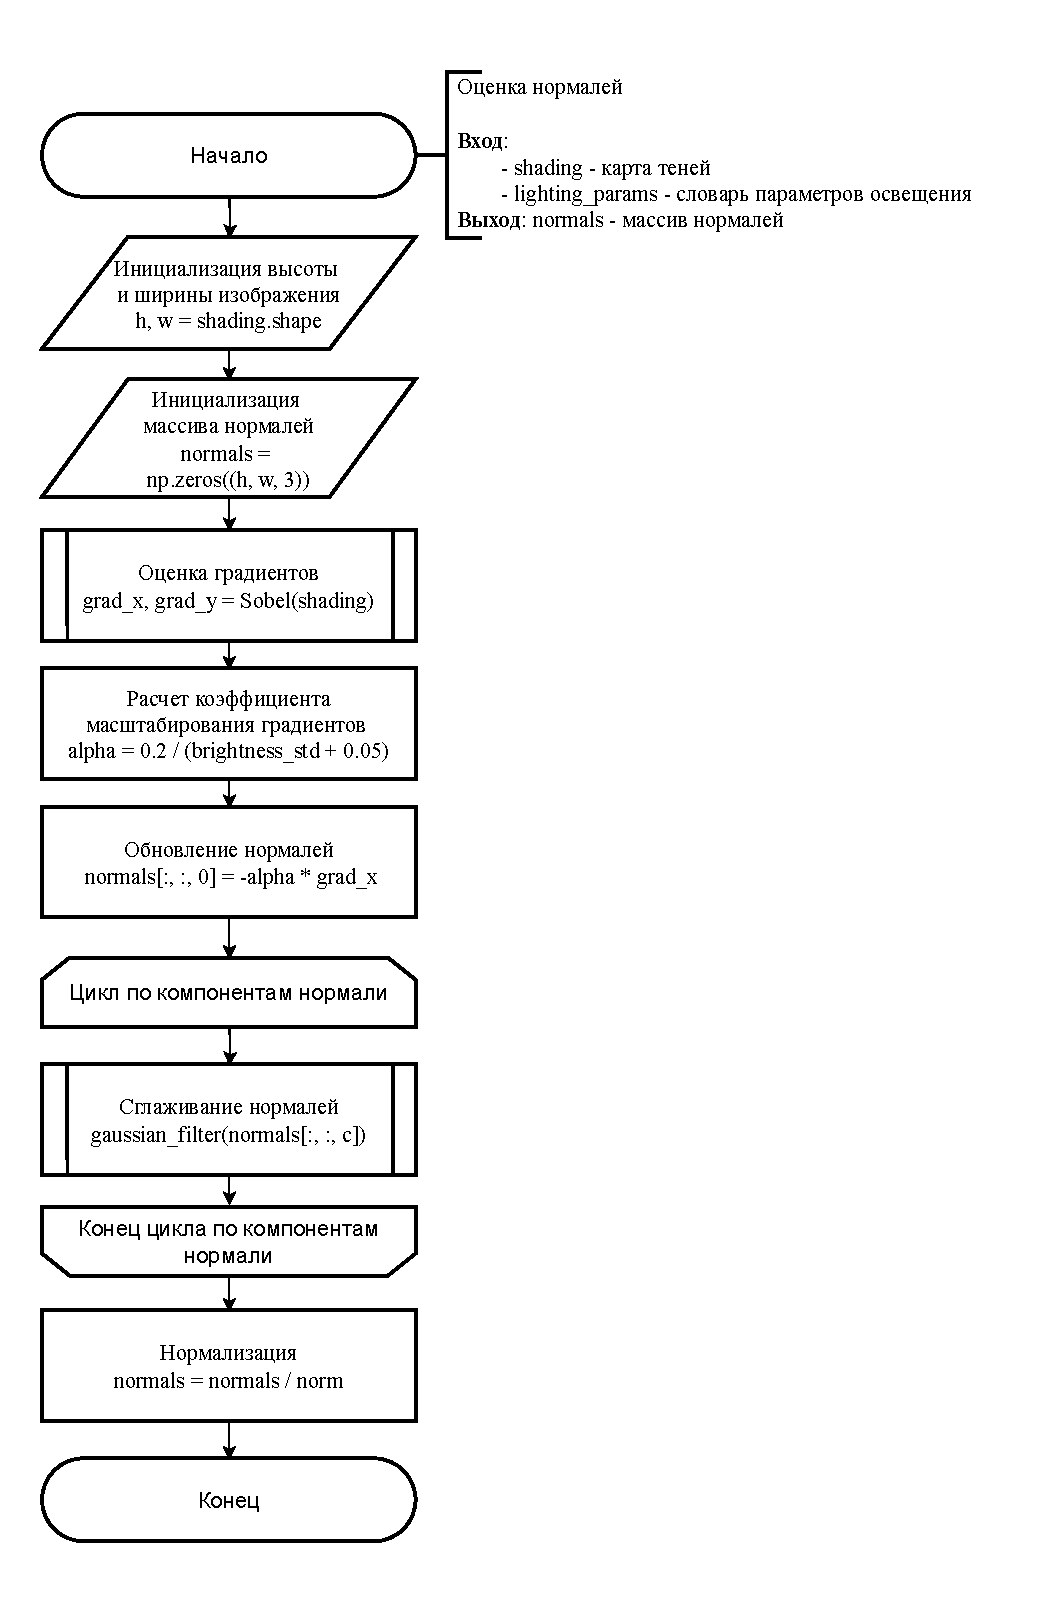
\includegraphics[scale=0.8]{img/normals}
    \caption{Оценка нормалей}
    \label{normals}
\end{figure}

Заключительный этап обработки представлен на рисунке~\ref{depth} --- алгоритм интеграции поля нормалей для получения итоговой карты глубин с высоким уровнем детализации поверхностей.

\begin{figure}[H]
    \centering
    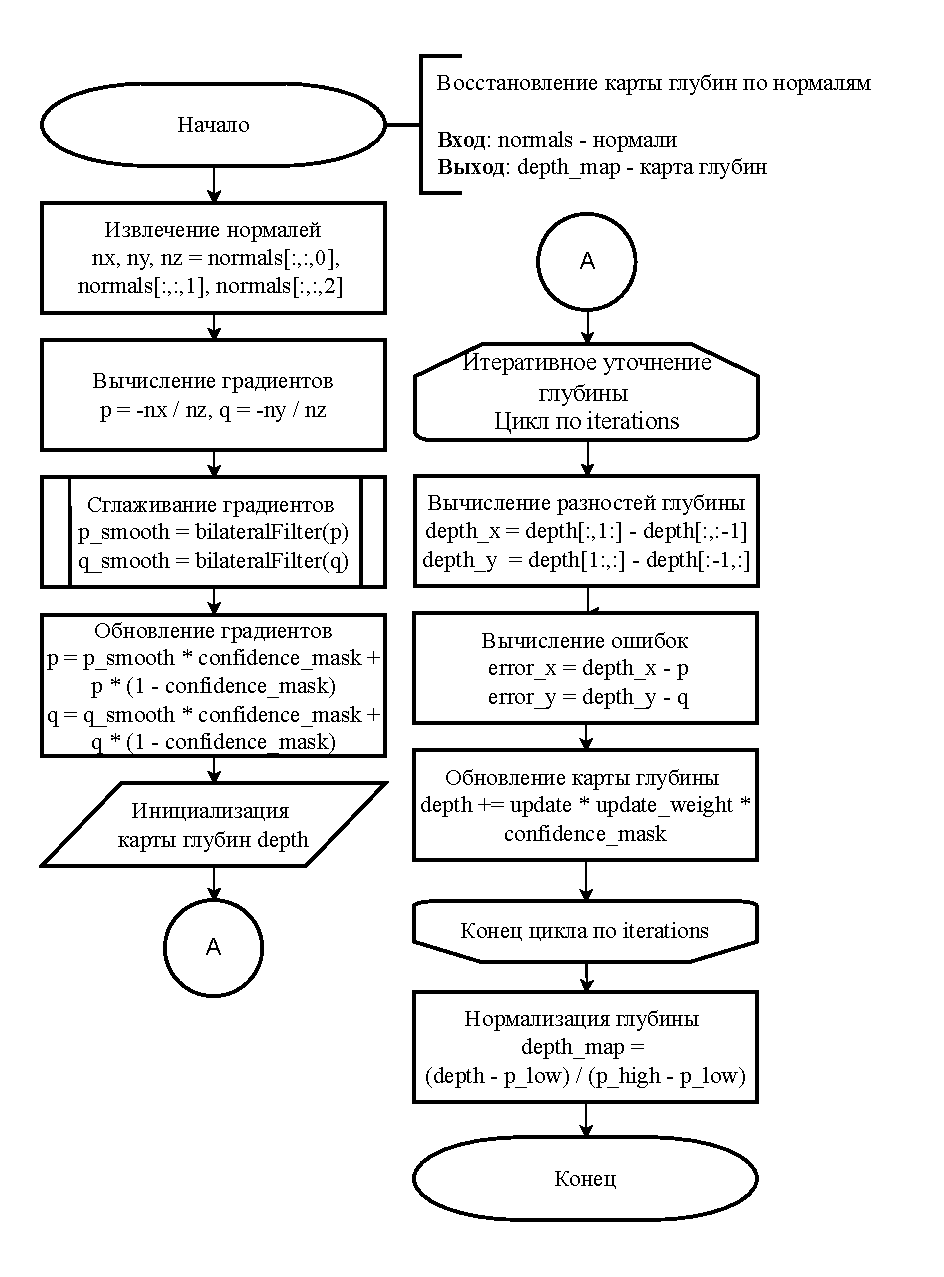
\includegraphics[scale=0.75]{img/depth}
    \caption{Восстановление карты глубин по нормалям}
    \label{depth}
\end{figure}

% TODO Надо добавить диаграмму компонентов разрабатываемого ПО?

\section*{Вывод}

В конструкторском разделе представлена детальная структура разработанного гибридного метода восстановления трехмерной информации из архивных фотографий.

Представленные схемы алгоритмов являются основой для последующей программной реализации метода, которая будет рассмотрена в технологическом разделе работы.
